% ============================================================
%  VisaPredict AI — Proyecto de Innovación Tecnológica I (PI-I)
%  Documento de desarrollo y validación del modelo predictivo.
%  Sigue el "Formato de seguimiento de avances del proyecto de
%  titulación" (MIAAD, UACJ) mapeado a la metodología CRISP-DM.
%  Compilar en Overleaf (igual que el Anteproyecto). Reutiliza el
%  preámbulo, paquetes y convenciones de AnteproyectoVisaPredictAI.tex.
% ============================================================
\documentclass[12pt,letterpaper]{report}

\usepackage[utf8]{inputenc}
\usepackage[T1]{fontenc}
\usepackage[spanish,es-tabla,es-nodecimaldot]{babel}
\usepackage{mathptmx}                     % Times New Roman
\usepackage{microtype}
\usepackage{ragged2e}
\usepackage[left=1.25in, right=1.25in, top=1in, bottom=1in]{geometry}
\usepackage{setspace}
\usepackage{graphicx}
\graphicspath{{Figures/}}
\usepackage{float}
\usepackage[table]{xcolor}
\usepackage{titlesec}
\usepackage{tocloft}
\usepackage{fancyhdr}
\usepackage[hyphens]{url}
\usepackage{hyperref}
\usepackage[nottoc]{tocbibind}
\usepackage{caption}
\captionsetup{justification=centering, font={small, color=gray}, labelfont={bf, color=gray}, format=plain}
\usepackage{enumitem}
\usepackage{multicol}
\usepackage{chngcntr}
\usepackage{tikz}
\usetikzlibrary{arrows.meta, positioning, fit, backgrounds}
\definecolor{uacjblue}{HTML}{003CA6}
\definecolor{uacjyellow}{HTML}{FFD600}
\definecolor{uacjgray}{HTML}{555559}
\definecolor{uacjblack}{HTML}{231F20}
\usepackage{amsmath}
\usepackage{amssymb}

% --- Interlineado y espaciado (idéntico al Anteproyecto) ---
\setstretch{1.10}
\setlength{\parskip}{0.4em}

% --- Numeración continua sin prefijo de capítulo ---
\renewcommand{\thetable}{\arabic{table}}
\renewcommand{\theequation}{\arabic{equation}}
\counterwithout{figure}{chapter}
\counterwithout{table}{chapter}
\counterwithout{equation}{chapter}
\setcounter{secnumdepth}{0}

\hypersetup{colorlinks=true, linkcolor=uacjblue, citecolor=uacjblue, urlcolor=uacjblue}

% --- Macro de citas IEEE clicables ---
\newcommand{\cita}[1]{\hyperref[bib:#1]{[#1]}}

\begin{document}

% ============================================================
% PORTADA (formato del seguimiento de avances)
% ============================================================
\begin{titlepage}
\centering
\begin{spacing}{1.2}
{\scshape\large Universidad Autónoma de Ciudad Juárez\par}
{\scshape Instituto de Ingeniería y Tecnología\par}
{\scshape Departamento de Ingeniería Eléctrica y Computación\par}
{\scshape Maestría en Inteligencia Artificial y Analítica de Datos\par}
\vspace{1.2cm}

\includegraphics[width=0.32\textwidth]{logouacj.png}\par
\vspace{1.2cm}
{\large\bfseries PREDICCIÓN DE FECHAS DE PRIORIDAD EN EL VISA BULLETIN DE
ESTADOS UNIDOS CONSIDERANDO PAÍS O ÁREA DE CARGABILIDAD, CATEGORÍA MIGRATORIA
Y TIPO DE TABLA\par}
\vspace{0.8cm}
{\itshape Desarrollo y validación de la propuesta de solución\par}
{\itshape Proyecto de Innovación Tecnológica I\par}
\vspace{1.4cm}
{Proyecto de innovación presentado por:\par}
{\bfseries Javier Augusto Rebull Saucedo \quad (263483)\par}
\vspace{0.8cm}
{Requisito para la obtención del título de\par}
{Maestro en Inteligencia Artificial y Analítica de Datos\par}
\vspace{1.0cm}
{Asesor:\par}
{\bfseries Dr. Vicente García Jiménez\par}
\vfill
{Ciudad Juárez, Chihuahua \hfill mayo de 2027\par}
\end{spacing}
\end{titlepage}

% ============================================================
% ÍNDICES
% ============================================================
\setlength{\parskip}{0pt}
\tableofcontents
\listoffigures
\listoftables
\setlength{\parskip}{0.4em}
\clearpage

% ============================================================
% 1. DESARROLLO DE LA PROPUESTA DE SOLUCIÓN
% ============================================================
\chapter{Desarrollo de la propuesta de solución}

La propuesta de solución es \textit{VisaPredict AI}, un sistema predictivo que
estima las fechas de prioridad del \textit{Visa Bulletin} del Departamento de
Estado de Estados Unidos, organizadas como un panel multiserie
$y_{p,c,b,t}$ indexado por país o área de cargabilidad $p$, categoría migratoria
$c$, tipo de tabla $b$ y mes $t$. El presente documento reporta la construcción y
la validación del modelo a partir del Anteproyecto, siguiendo las fases de la
metodología \textit{Cross-Industry Standard Process for Data Mining} (CRISP-DM)
\cita{1}: comprensión y preparación de los datos, modelado y evaluación.

El sistema opera como un regresor temporal único entrenado exclusivamente sobre
las observaciones con fecha publicada (estado $e=F$). Las celdas con régimen
\textit{Current} ($C$) o \textit{Unavailable} ($U$) se conservan como anotación
descriptiva, pero no son objetivo predictivo: el sistema no promete anticipar los
cambios de régimen. Las tablas \textit{Final Action Dates} (FAD) y \textit{Dates
for Filing} (DFF) se modelan y se evalúan por separado.

La arquitectura sigue un flujo modular que transforma el almacén de datos en
pronósticos con intervalos de predicción. En la Figura~\ref{fig:arquitectura} se
muestra el esquema. El sistema consta de cinco módulos:

\begin{enumerate}[leftmargin=*]
\item \textbf{Carga de series.} Lee del almacén dimensional (capa \textit{gold},
DuckDB) la vista entrenable, que ya restringe las observaciones a $e=F$ y separa
FAD de DFF. Entrega cada serie $y_{p,c,b,t}$ con índice mensual.
\item \textbf{Preprocesamiento.} Regulariza la frecuencia mensual, interpola los
huecos cortos (meses $C$/$U$ intercalados) y deja como faltantes los huecos
largos; estandariza con estadísticos calculados solo sobre el tramo de
entrenamiento y construye los regresores de calendario del año fiscal.
\item \textbf{Catálogo de modelos.} Ocho modelos de referencia tras una interfaz
común: naïve estacional, ARIMA, SARIMA, Prophet, LSTM, DeepAR, la cascada
ARIMA-LSTM y XGBoost con regresores.
\item \textbf{Validación walk-forward.} Validación temporal con ventana
expansible y paso mensual que evalúa cada modelo sin fuga de información, reservando
los últimos 24 meses como conjunto independiente.
\item \textbf{Cuantificación de incertidumbre.} Genera intervalos de predicción al
95\,\% por dos mecanismos (probabilístico nativo y conforme dividido) y reporta su
cobertura empírica.
\end{enumerate}

\begin{figure}[H]
\centering
\begin{tikzpicture}[
  font=\footnotesize,
  box/.style={rectangle, rounded corners=2pt, draw=uacjblue, line width=0.6pt,
    fill=white, text width=2.5cm, align=center, minimum height=1.1cm,
    inner sep=3pt, outer sep=0pt},
  store/.style={box, fill=uacjblue!10},
  arr/.style={-{Latex[length=2mm]}, uacjgray, line width=0.7pt}]
  \node[store] (db) {Almacén DuckDB (vista entrenable $e=F$)};
  \node[box, right=0.6cm of db] (pre) {Preprocesa\-miento (huecos, escala, calendario)};
  \node[box, right=0.6cm of pre] (mod) {Catálogo de 8 modelos};
  \node[box, right=0.6cm of mod] (wf) {Walk-forward (holdout 24 m)};
  \node[box, fill=uacjyellow!25, right=0.6cm of wf] (pi) {Pronóstico + intervalo 95\,\%};
  \draw[arr] (db) -- (pre);
  \draw[arr] (pre) -- (mod);
  \draw[arr] (mod) -- (wf);
  \draw[arr] (wf) -- (pi);
\end{tikzpicture}
\caption[Arquitectura del sistema de modelado]{Flujo modular de VisaPredict AI:
del almacén entrenable al pronóstico con intervalo de predicción al 95\,\%.}
\label{fig:arquitectura}
\end{figure}

% ------------------------------------------------------------
\section{1.1 Recolección de datos}

Esta sección recapitula la fase de comprensión y adquisición de los datos,
construida como Objetivo~1 del proyecto. Se describen las fuentes y el proceso de
obtención y conversión al formato de modelado.

\subsection{1.1.1 Identificación de fuentes de datos}

La fuente primaria es el \textit{Visa Bulletin} mensual publicado por el
Departamento de Estado de Estados Unidos en \texttt{travel.state.gov}. Su elección
obedece a tres criterios: es la fuente oficial y autoritativa de las fechas de
prioridad; cubre de forma homogénea las cinco áreas de cargabilidad de interés
(México, India, China, Filipinas y \textit{All Chargeability Areas Except Those
Listed}); y publica de manera consistente las dos tablas relevantes, FAD y DFF.
Para asegurar la reproducibilidad y la resiliencia ante la rotación de boletines
viejos del portal oficial, cada boletín se congela como instantánea HTML en un
respaldo versionado, del cual el procesamiento parte de forma reproducible.

\subsection{1.1.2 Obtención de los datos y conversión al formato adecuado}

La extracción se realiza por \textit{web scraping} de las instantáneas congeladas,
con una detección de columnas robusta a veinte años de deriva de formato. El dato
crudo de cada celda se conserva tal cual se publicó y se clasifica en el régimen
$e \in \{F, C, U, \text{UNK}\}$. La variable dependiente $y_{p,c,b,t}$ se define
como el número de días desde la época base $t_0 = $ 1-ene-1975, calculado solo para
las celdas con fecha ($e=F$).

Los datos se consolidan en un panel largo y se cargan en un almacén dimensional en
estrella (DuckDB) cuyas restricciones de clave e integridad actúan como contrato de
calidad. El conjunto resultante comprende \textbf{194 series} y \textbf{27{,}277
filas} en el rango \textbf{dic-2001 a 2026}, con una cobertura a nivel de boletín
del 98.3\,\% (291 de 296 meses; los cinco ausentes no existen en la fuente oficial).
Los principales retos enfrentados fueron: la heterogeneidad del formato HTML a lo
largo de dos décadas; la distinción entre "sin dato" y "Unavailable" (resuelta con
el centinela \texttt{UNK} en lugar de \texttt{NA}, que colisiona con la coerción de
\texttt{pandas}); y la naturaleza dispersa de las series, pues los meses en régimen
$C$ o $U$ no aportan fecha y se manifiestan como huecos.

% ------------------------------------------------------------
\section{1.2 Análisis de datos}

Se caracterizan las series antes de modelar y se documentan las transformaciones
aplicadas.

\subsection{1.2.1 Análisis exploratorio de datos (EDA)}

El EDA cubre las 25 series FAD de preferencia familiar de las cinco áreas piloto.
La Figura~\ref{fig:eda_pilot} muestra la categoría F3 a través de las cinco áreas:
\textit{All Chargeability} avanza de forma suave y casi monótona, mientras que
México y Filipinas exhiben retrocesos pronunciados (retrogresiones) concentrados
entre 2002 y 2008, evidencia directa de la heterogeneidad por país-categoría.

\begin{figure}[H]
\centering
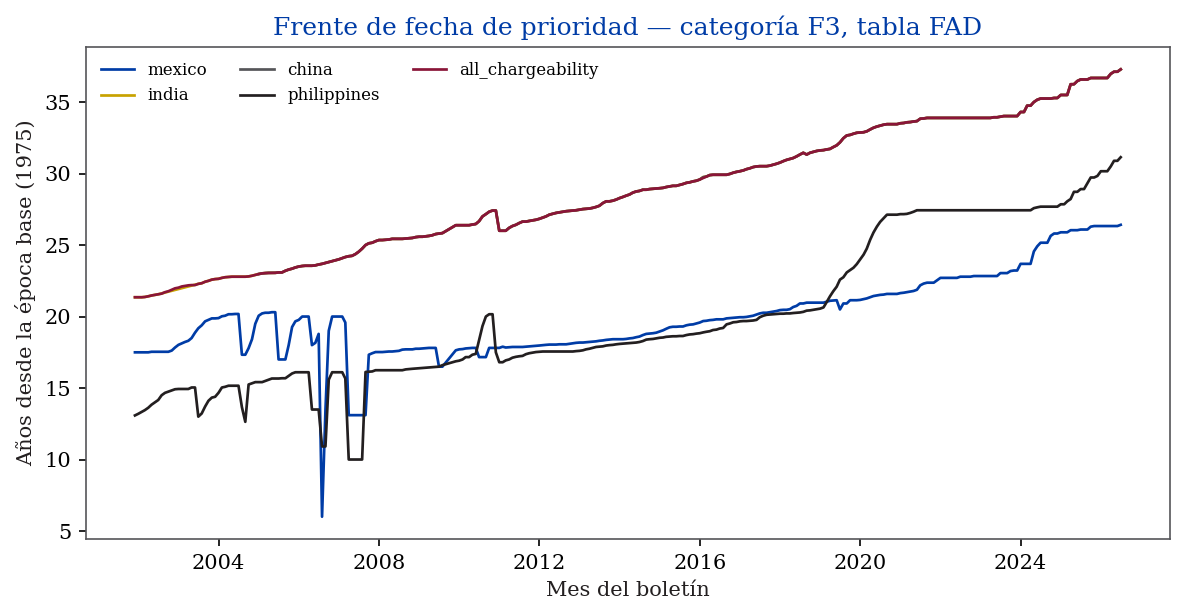
\includegraphics[width=0.92\textwidth]{eda_pilot_F3_FAD.png}
\caption[Frente de fecha de prioridad por área]{Categoría F3, tabla FAD, a través de
las cinco áreas piloto. La pendiente y los retrocesos difieren marcadamente por
área.}
\label{fig:eda_pilot}
\end{figure}

La Figura~\ref{fig:eda_coverage} resume la continuidad de las series (fracción de
meses con fecha publicada). La categoría F2A presenta la menor continuidad
($\approx$80\,\%) porque transita con frecuencia al régimen \textit{Current}. La
Figura~\ref{fig:eda_steps} muestra la distribución del avance mensual: la masa se
concentra en avances pequeños y positivos, con una cola izquierda que corresponde a
las retrogresiones que el modelo debe tolerar.

\begin{figure}[H]
\centering
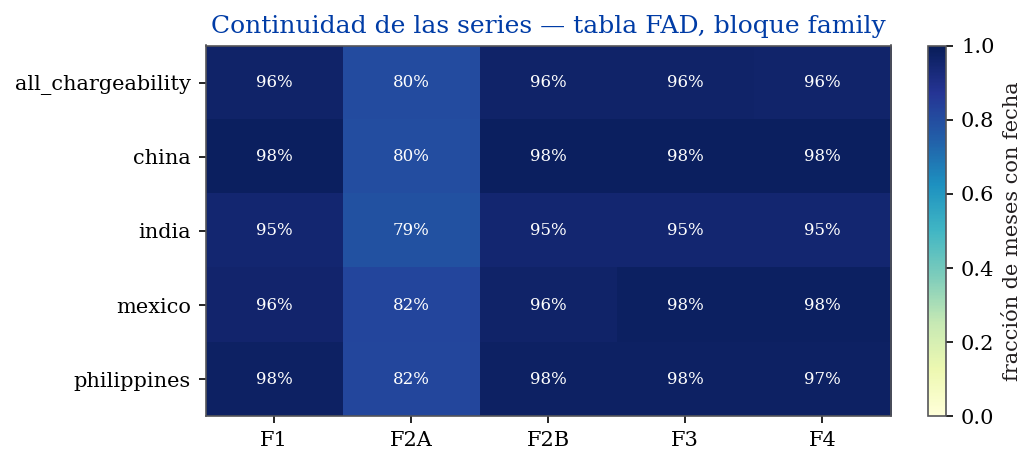
\includegraphics[width=0.85\textwidth]{eda_coverage_FAD_family.png}
\caption[Continuidad de las series]{Fracción de meses con fecha publicada por área y
categoría (tabla FAD, preferencia familiar).}
\label{fig:eda_coverage}
\end{figure}

\begin{figure}[H]
\centering
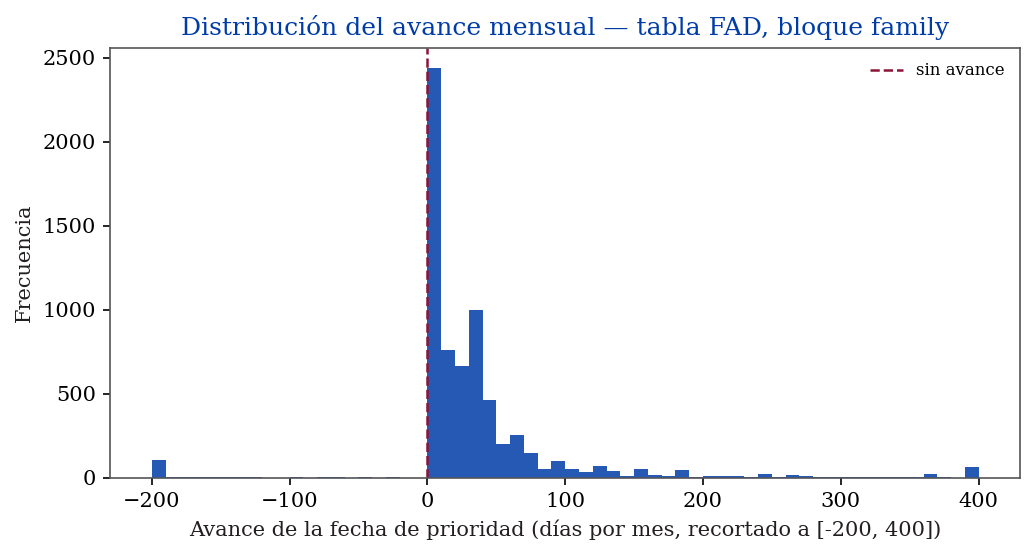
\includegraphics[width=0.78\textwidth]{eda_steps_FAD_family.png}
\caption[Distribución del avance mensual]{Avance mensual de la fecha de prioridad;
la cola izquierda corresponde a las retrogresiones.}
\label{fig:eda_steps}
\end{figure}

La descomposición STL de una serie representativa (Figura~\ref{fig:eda_stl})
confirma una tendencia creciente dominante y una componente estacional pequeña,
con residuos volátiles concentrados en el periodo temprano. Las pruebas de
estacionariedad lo formalizan: para la serie México/F3/FAD, la prueba de
\textit{Augmented Dickey-Fuller} (ADF) no rechaza la raíz unitaria ($p=0.99$) y la
de \textit{Kwiatkowski-Phillips-Schmidt-Shin} (KPSS) rechaza la estacionariedad en
nivel ($p<0.01$); ambas concuerdan en que la serie requiere una diferenciación. Como
la prueba ADF pierde potencia precisamente bajo tendencia fuerte y muestras cortas
—el escenario de este panel—, se añade la prueba DF-GLS de Elliott-Rothenberg-Stock
\cita{15}, que aplica un \textit{detrending} por mínimos cuadrados generalizados y
alcanza la envolvente de potencia óptima; también confirma la no estacionariedad en
nivel ($p=0.78$), reforzando de forma más robusta la elección $d=1$. La
Figura~\ref{fig:eda_acf} muestra la autocorrelación de la serie diferenciada, que
orienta el orden de los modelos ARIMA y SARIMA.

\begin{figure}[H]
\centering
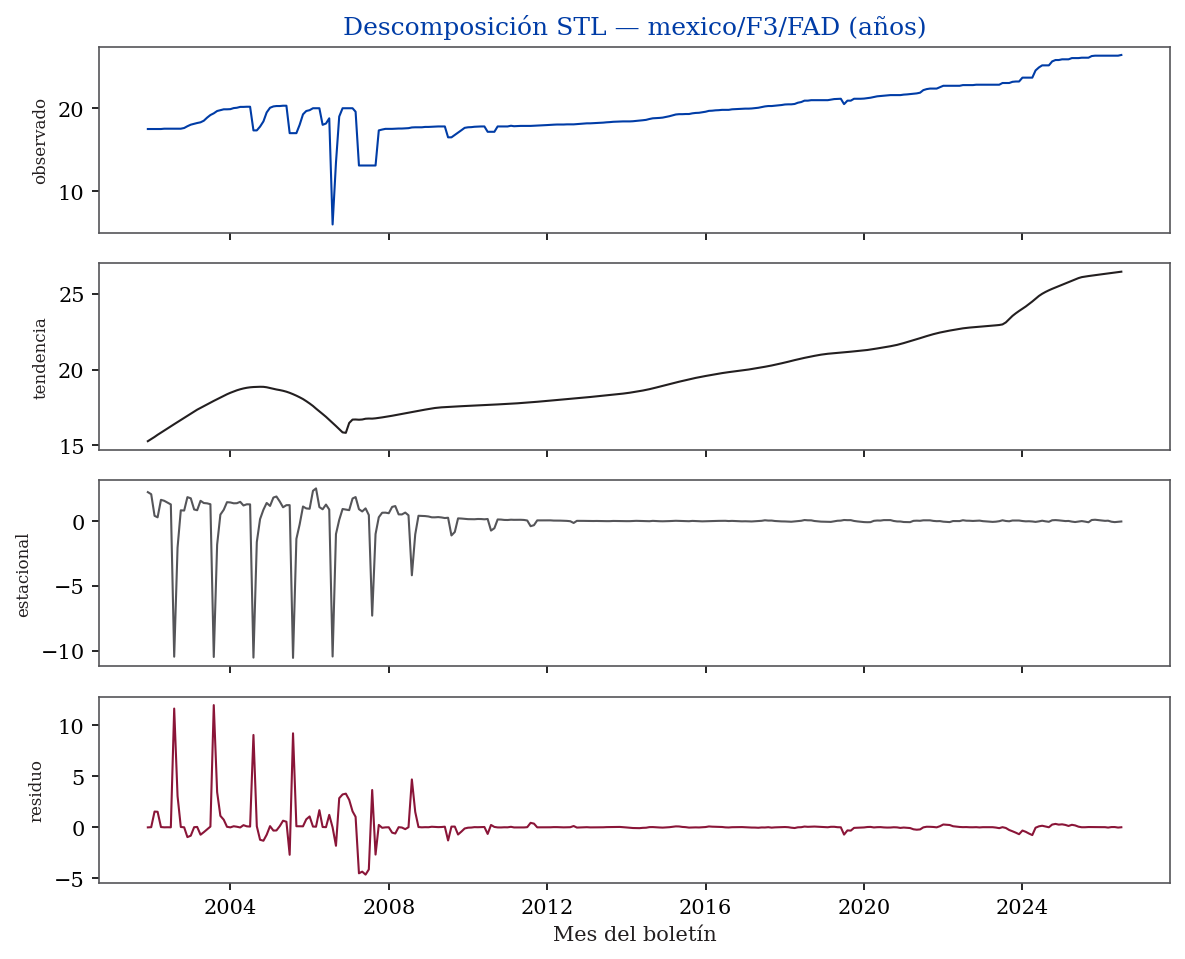
\includegraphics[width=0.85\textwidth]{eda_stl_mexico_F3_FAD.png}
\caption[Descomposición STL]{Descomposición STL de México/F3/FAD en tendencia,
componente estacional y residuo (en años).}
\label{fig:eda_stl}
\end{figure}

\begin{figure}[H]
\centering
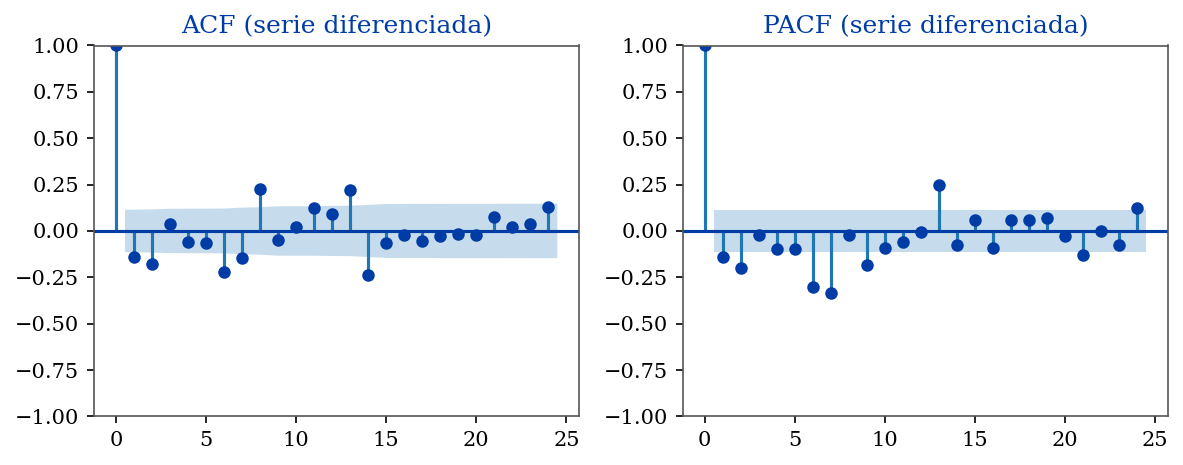
\includegraphics[width=0.85\textwidth]{eda_acfpacf_mexico_F3_FAD.png}
\caption[ACF y PACF]{Funciones de autocorrelación (ACF) y autocorrelación parcial
(PACF) de la serie diferenciada México/F3/FAD.}
\label{fig:eda_acf}
\end{figure}

\subsubsection{Catálogo de características por serie}

Examinar 25 series una por una no escala. Por ello se adopta el enfoque de análisis
basado en características (\textit{feature-based}) \cita{10}: se resume cada serie en
un vector de descriptores numéricos comparables, de modo que el panel completo se
analiza como una tabla. A continuación se define cada característica, su rango y su
lectura operativa para el modelado.

\paragraph{Fuerza de tendencia y de estacionalidad ($F_T$, $F_S$).} A partir de la
descomposición STL $Y_t = T_t + S_t + R_t$ (tendencia, estacionalidad, residuo) se
miden, según la formulación de descomposición de FPP3,
\begin{equation}
F_T = \max\!\left(0,\; 1 - \frac{\operatorname{Var}(R_t)}{\operatorname{Var}(T_t + R_t)}\right),
\qquad
F_S = \max\!\left(0,\; 1 - \frac{\operatorname{Var}(R_t)}{\operatorname{Var}(S_t + R_t)}\right).
\end{equation}
Ambas viven en $[0,1]$: un valor cercano a 1 indica que la tendencia (resp. la
estacionalidad) explica casi toda la variación más allá del ruido; cercano a 0, que
es despreciable.

\paragraph{Entropía espectral ($H$).} Mide qué tan concentrado está el espectro de la
serie. Sobre el periodograma normalizado $\{p_k\}$ (densidad espectral que suma 1),
\begin{equation}
H = \frac{-\sum_k p_k \log p_k}{\log K},
\end{equation}
con $K$ el número de frecuencias. $H \to 0$ señala una señal muy estructurada y
predecible; $H \to 1$, ruido blanco sin estructura aprovechable.

\paragraph{Autocorrelación (ACF1, $ACF1_\Delta$).} ACF1 es la autocorrelación de
rezago 1 del nivel; $ACF1_\Delta$, la de la serie diferenciada. Un ACF1 cercano a 1
confirma alta persistencia (memoria larga); el signo de $ACF1_\Delta$ orienta el
término de media móvil de un ARIMA.

\paragraph{Orden de diferenciación ($d$).} Número de diferencias necesarias para
estacionariedad, determinado de forma iterativa con la prueba KPSS (FPP3 §9.1):
mientras KPSS rechace la estacionariedad, se diferencia y se reintenta. Alimenta
directamente el parámetro $d$ de ARIMA.

\paragraph{Atípicos.} Número de residuos de la STL cuyo $z$-score robusto (basado en
la mediana y la desviación absoluta mediana, criterio de Iglewicz-Hoaglin) supera 3
en valor absoluto. Cuantifica la carga de anomalías —en este dominio, las
retrogresiones.

\paragraph{Ruido blanco (Ljung-Box, LB\,$p$).} P-valor de la prueba de Ljung-Box
sobre $2m=24$ rezagos (FPP3 §2.9); la hipótesis nula es que la serie es ruido blanco.
Un $p$ pequeño confirma que queda estructura temporal modelable.

\paragraph{Asimetría y curtosis.} Sobre la distribución de los avances mensuales:
la asimetría capta el sesgo (las retrogresiones producen colas izquierdas) y la
curtosis, el peso de las colas (eventos extremos).

Las Tablas~\ref{tab:features_estructura} y~\ref{tab:features_anomalias} reportan estos
descriptores para las 25 series. Las medidas de estabilidad y \textit{lumpiness}
(varianza de medias y de varianzas por bloque) se calculan en el módulo pero se omiten
de las tablas por ser dependientes de la escala en días; quedan en el registro
reproducible.

\begin{table}[H]
\centering
\footnotesize
\caption[Características estructurales de las series]{Estructura temporal de las 25 series FAD de preferencia familiar. $F_T$/$F_S$: fuerza de tendencia y estacionalidad; $H$: entropía espectral; $d$: orden de diferenciación.}
\label{tab:features_estructura}
\begin{tabular}{llcccccc}
\hline
\rowcolor{uacjblue!15}
\textbf{Área} & \textbf{Cat.} & $\mathbf{F_T}$ & $\mathbf{F_S}$ & $\mathbf{H}$ & \textbf{ACF1} & $\mathbf{ACF1_\Delta}$ & $\mathbf{d}$ \\ \hline
CN & F1 & 0.993 & 0.001 & 0.292 & 0.989 & +0.276 & 1 \\
CN & F2A & 0.991 & 0.000 & 0.338 & 0.987 & +0.158 & 1 \\
CN & F2B & 0.998 & 0.029 & 0.299 & 0.989 & +0.269 & 1 \\
CN & F3 & 0.998 & 0.000 & 0.344 & 0.987 & +0.114 & 1 \\
CN & F4 & 0.993 & 0.024 & 0.351 & 0.984 & -0.216 & 1 \\
IN & F1 & 0.990 & 0.000 & 0.301 & 0.990 & +0.208 & 1 \\
IN & F2A & 0.994 & 0.007 & 0.319 & 0.989 & +0.160 & 1 \\
IN & F2B & 0.998 & 0.030 & 0.271 & 0.992 & +0.251 & 1 \\
IN & F3 & 0.999 & 0.000 & 0.332 & 0.989 & +0.118 & 1 \\
IN & F4 & 0.993 & 0.000 & 0.335 & 0.988 & -0.060 & 1 \\
MX & F1 & 0.928 & 0.227 & 0.407 & 0.956 & +0.045 & 2 \\
MX & F2A & 0.995 & 0.066 & 0.305 & 0.990 & +0.142 & 1 \\
MX & F2B & 0.997 & 0.074 & 0.356 & 0.985 & +0.104 & 2 \\
MX & F3 & 0.754 & 0.000 & 0.445 & 0.918 & -0.142 & 1 \\
MX & F4 & 0.958 & 0.136 & 0.411 & 0.972 & -0.019 & 1 \\
PH & F1 & 0.990 & 0.000 & 0.251 & 0.991 & +0.117 & 1 \\
PH & F2A & 0.994 & 0.008 & 0.319 & 0.989 & +0.159 & 1 \\
PH & F2B & 0.995 & 0.024 & 0.276 & 0.990 & +0.158 & 1 \\
PH & F3 & 0.967 & 0.074 & 0.330 & 0.981 & +0.075 & 1 \\
PH & F4 & 0.997 & 0.000 & 0.322 & 0.989 & +0.229 & 1 \\
RoW & F1 & 0.991 & 0.011 & 0.296 & 0.989 & +0.202 & 1 \\
RoW & F2A & 0.994 & 0.007 & 0.319 & 0.989 & +0.160 & 1 \\
RoW & F2B & 0.999 & 0.033 & 0.271 & 0.992 & +0.276 & 1 \\
RoW & F3 & 0.999 & 0.000 & 0.331 & 0.989 & +0.120 & 1 \\
RoW & F4 & 0.997 & 0.170 & 0.327 & 0.988 & -0.232 & 1 \\
\hline
\end{tabular}
\end{table}

\begin{table}[H]
\centering
\footnotesize
\caption[Anomalías y forma de las series]{Anomalías y forma de la distribución de los avances. Atípicos: residuos STL con $|z|>3$; LB$\,p$: p-valor de Ljung-Box (H0 ruido blanco); asimetría y curtosis de los avances mensuales.}
\label{tab:features_anomalias}
\begin{tabular}{llcccc}
\hline
\rowcolor{uacjblue!15}
\textbf{Área} & \textbf{Cat.} & \textbf{Atípicos} & \textbf{LB}\,$p$ & \textbf{Asim.} & \textbf{Curt.} \\ \hline
CN & F1 & 68 & 0.000 & -2.85 & 55.2 \\
CN & F2A & 66 & 0.000 & -3.64 & 30.9 \\
CN & F2B & 32 & 0.000 & -6.74 & 95.8 \\
CN & F3 & 40 & 0.000 & -5.76 & 84.4 \\
CN & F4 & 42 & 0.000 & -2.28 & 55.0 \\
IN & F1 & 70 & 0.000 & -5.15 & 60.2 \\
IN & F2A & 68 & 0.000 & -3.88 & 35.7 \\
IN & F2B & 34 & 0.000 & -6.68 & 100.8 \\
IN & F3 & 44 & 0.000 & -6.05 & 95.1 \\
IN & F4 & 45 & 0.000 & -3.10 & 48.8 \\
MX & F1 & 76 & 0.000 & -2.63 & 100.1 \\
MX & F2A & 80 & 0.000 & -5.78 & 76.8 \\
MX & F2B & 75 & 0.000 & +0.66 & 21.8 \\
MX & F3 & 78 & 0.000 & -4.81 & 79.4 \\
MX & F4 & 65 & 0.000 & -3.39 & 78.9 \\
PH & F1 & 73 & 0.000 & -6.24 & 57.2 \\
PH & F2A & 67 & 0.000 & -3.88 & 35.6 \\
PH & F2B & 68 & 0.000 & -4.04 & 66.4 \\
PH & F3 & 78 & 0.000 & +0.88 & 48.2 \\
PH & F4 & 62 & 0.000 & -7.65 & 107.1 \\
RoW & F1 & 61 & 0.000 & -4.00 & 50.9 \\
RoW & F2A & 72 & 0.000 & -3.88 & 35.6 \\
RoW & F2B & 33 & 0.000 & -7.03 & 106.9 \\
RoW & F3 & 44 & 0.000 & -6.05 & 94.9 \\
RoW & F4 & 51 & 0.000 & -2.60 & 74.7 \\
\hline
\end{tabular}
\end{table}


\paragraph{Lectura de la Tabla~\ref{tab:features_estructura} (estructura).} El panel
es notablemente homogéneo: la fuerza de tendencia $F_T$ supera 0.99 en la mayoría de
las series, con las únicas excepciones de las series mexicanas y filipinas más
volátiles (MX/F3 con $F_T=0.754$, MX/F1 con $0.928$, PH/F3 con $0.967$). La fuerza de
estacionalidad $F_S$ es prácticamente nula en todo el panel ($F_S < 0.23$, con muchas
series exactamente en 0), lo que confirma que las fechas de prioridad \textbf{no
tienen un ciclo anual relevante}; este es el hallazgo que explica por qué los términos
estacionales de SARIMA no mejoran a ARIMA en los resultados. La autocorrelación de
nivel ACF1 ronda 0.98--0.99 (persistencia alta, coherente con la tendencia), y el
orden de diferenciación es $d=1$ salvo dos series mexicanas que requieren $d=2$. La
Figura~\ref{fig:eda_features} visualiza esta homogeneidad: todas las series se agrupan
en la esquina de tendencia fuerte y estacionalidad casi nula.

\begin{figure}[H]
\centering
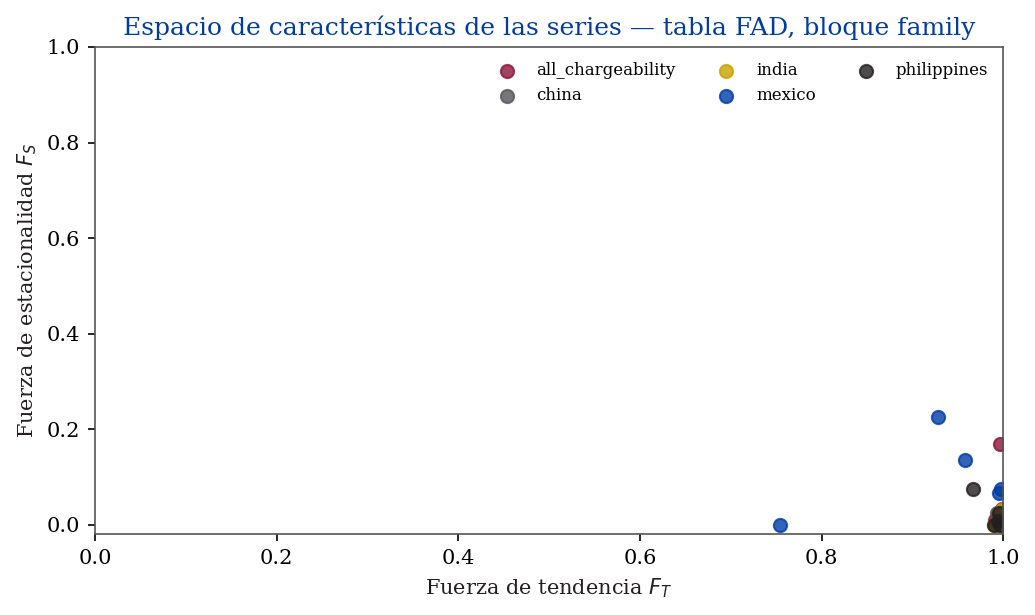
\includegraphics[width=0.82\textwidth]{eda_features_FAD_family.png}
\caption[Espacio de características]{Cada serie como un punto en el plano fuerza de
tendencia--fuerza de estacionalidad. El panel es homogéneo: tendencia fuerte y
estacionalidad casi nula.}
\label{fig:eda_features}
\end{figure}

\paragraph{Lectura de la Tabla~\ref{tab:features_anomalias} (anomalías y forma).} La
prueba de Ljung-Box rechaza el ruido blanco en las 25 series ($p < 0.001$ en todas):
hay estructura temporal que un modelo puede aprovechar. La distribución de los avances
es marcadamente no gaussiana: la asimetría es casi siempre negativa (las
retrogresiones generan colas izquierdas) y la curtosis es extrema —entre 22 y 107—,
lo que señala eventos atípicos frecuentes.

\subsubsection{Cambios de régimen frente a anomalías puntuales}

El conteo de la columna ``Atípicos'' (32--80) proviene de un $z$-score robusto por
punto y, por sí solo, confunde dos fenómenos distintos. Un diagnóstico de mayor nivel
los separa: por un lado, los \textbf{cambios de régimen} —desplazamientos estructurales
duraderos— se detectan con el algoritmo PELT (\textit{Pruned Exact Linear Time})
\cita{12} sobre la serie estandarizada; por otro, las \textbf{anomalías puntuales}
—observaciones aisladas— con un filtro de Hampel sobre el residuo de la STL (mediana y
MAD locales). Aplicado a México/F3/FAD, el método identifica \textbf{solo 3 cambios de
régimen} (no 78), mientras que las anomalías puntuales se concentran en la era volátil
2002--2008 (Figura~\ref{fig:eda_changepoints}). La consecuencia para el modelado es
precisa: el grueso de la ``rareza'' de estas series es estructural (regímenes), no
ruido aislado, por lo que la validación debe usar métricas robustas y los modelos,
tolerar retrogresiones sostenidas.

\begin{figure}[H]
\centering
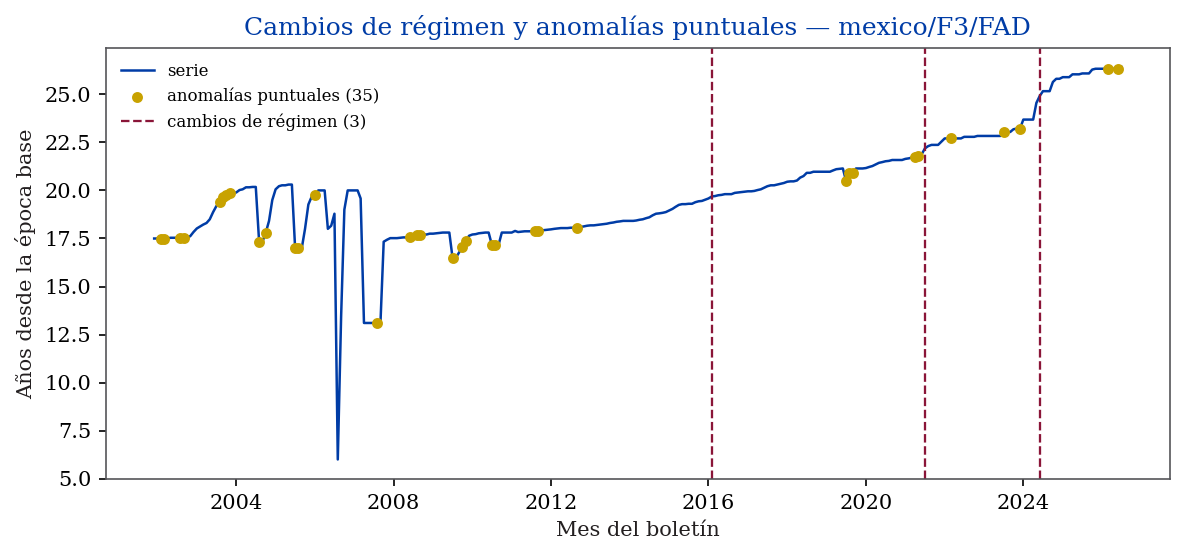
\includegraphics[width=0.86\textwidth]{eda_changepoints_mexico_F3_FAD.png}
\caption[Cambios de régimen y anomalías puntuales]{Cambios de régimen (PELT, líneas
verticales) frente a anomalías puntuales (filtro de Hampel, marcadores) en
México/F3/FAD. Distingue desplazamientos estructurales de observaciones aisladas.}
\label{fig:eda_changepoints}
\end{figure}

\paragraph{Diagnósticos avanzados de complejidad y memoria.} Para completar la
caracterización se calcula, por serie, el exponente de Hurst (mediante análisis de
fluctuación sin tendencia), la entropía de permutación y de muestra, la $\lambda$
óptima de Box-Cox y la prueba de Zivot-Andrews (raíz unitaria con un quiebre endógeno),
además del conjunto canónico de 22 características \textit{catch22} \cita{11}, un
subconjunto de alto rendimiento seleccionado entre más de siete mil descriptores. En
México/F3/FAD el exponente de Hurst supera 1 (memoria larga, fuertemente persistente),
las entropías de permutación y de muestra son bajas ($\approx 0.13$--$0.17$, señal de
una dinámica muy regular y por tanto predecible), la $\lambda$ de Box-Cox queda cerca
de 1 (no se requiere transformar la varianza) y Zivot-Andrews rechaza la raíz unitaria
tras una diferencia ($p < 0.001$), reforzando la elección $d=1$. Finalmente, la prueba
BDS de Brock-Dechert-Scheinkman-LeBaron \cita{18} —cuya hipótesis nula es que la serie
diferenciada es independiente e idénticamente distribuida— se rechaza con fuerza
($p < 0.001$), lo que evidencia dependencia no lineal y justifica de forma cuantitativa
incluir modelos no lineales (LSTM, DeepAR, XGBoost) en la comparación, en lugar de
hacerlo por defecto.

\subsubsection{Selección y des-redundancia de características}

Con muestras de 125 a 290 observaciones por serie, cada grado de libertad cuenta, por
lo que el conjunto unido de características (catch22, descriptores de pronóstico y
variables de dominio) se somete a una etapa formal de selección en dos pasos. Primero,
un filtro de relevancia univariada con corrección de multiplicidad de Benjamini-Yekutieli
—el patrón del algoritmo FRESH \cita{14}— que controla la tasa de falso descubrimiento.
Segundo, una des-redundancia por correlación de Spearman —en el espíritu de la selección
de mínima redundancia y máxima relevancia (mRMR) \cita{16}— que conserva una sola
característica representativa de cada grupo colineal; esto resuelve, por ejemplo, la
duplicación entre el exponente de Hurst y las características de escalamiento de catch22.
Para evitar fuga de información, la selección se ajusta únicamente con datos de
entrenamiento dentro de cada partición del walk-forward. La decisión de no apilar
bibliotecas completas de características (que serían cientos, con fuerte redundancia
mutua) se apoya en la evidencia empírica de redundancia entre conjuntos de
características \cita{17}: pocos descriptores bien elegidos superan a muchos correlacionados.

\subsubsection{Métodos del estado del arte evaluados y descartados por diagnóstico}

Una revisión amplia de la literatura confirmó que varias familias de técnicas en boga
\textit{no aplican} a este problema, y descartarlas con criterio es parte del análisis.
La descomposición estacional múltiple (MSTL) y las pruebas de raíz unitaria estacional
(HEGY, OCSB) son innecesarias porque la estacionalidad es prácticamente nula ($F_S<0.25$).
El exponente de Hurst mayor que 1 indica no estacionariedad pura, no memoria larga
fraccional, por lo que los modelos ARFIMA y los estimadores de tipo GPH son
inapropiados. La familia de descomposición empírica (EMD, EEMD, CEEMDAN) y de
\textit{wavelets} usada como ``descomponer y luego pronosticar'' es notoria por inflar
la exactitud mediante fuga de información hacia el futuro, incompatible con la validación
walk-forward de este trabajo. Las representaciones modernas por convoluciones aleatorias
(ROCKET y variantes), \textit{shapelets} y diccionarios simbólicos (BOSS, WEASEL) están
diseñadas para la \textit{clasificación} de series como objetos, no para la regresión
temporal autorregresiva de un panel; y las firmas de camino (\textit{path signatures})
aportan sobre todo en escenarios multivariados, mientras que aquí el objetivo es
univariado. Documentar estas exclusiones evita la falsa impresión de carencia: son
decisiones fundamentadas, no omisiones.

\paragraph{Estructura cruzada del panel.} Como el objetivo es un panel multiserie, se
examina además el co-movimiento entre áreas. La Figura~\ref{fig:eda_cross} muestra la
correlación de los avances mensuales entre las cinco áreas para la categoría F3:
India, China y \textit{All Chargeability} se mueven casi al unísono (correlación
$\approx 1$), pues comparten el frente mundial cuando no están rezagadas, mientras que
México y Filipinas evolucionan de forma independiente por sus rezagos propios. Esta
separación entre un grupo ``mundial'' y series país-específicas respalda la
heterogeneidad por país-categoría y orienta posibles modelos globales que compartan
información dentro del grupo mundial.

\begin{figure}[H]
\centering
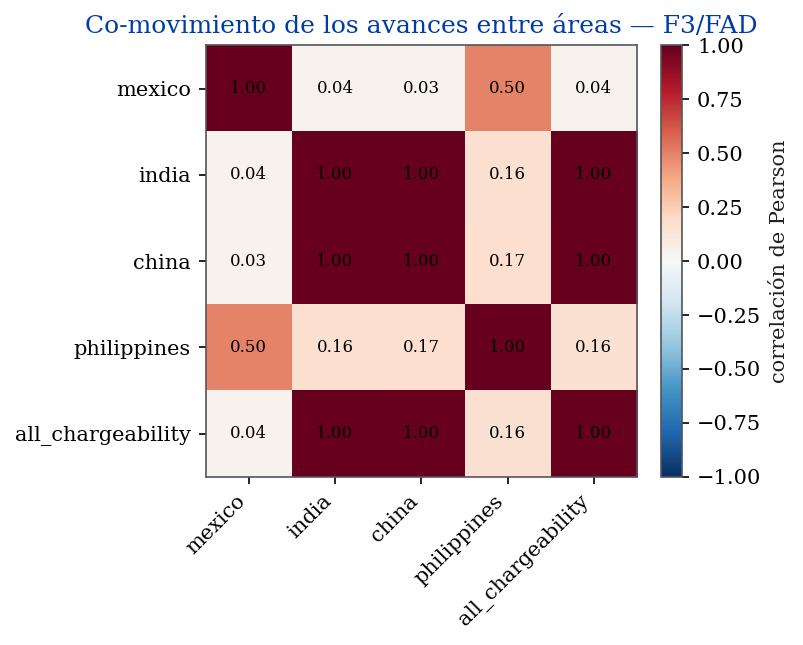
\includegraphics[width=0.62\textwidth]{eda_crosscorr_F3_FAD.png}
\caption[Co-movimiento entre áreas]{Correlación de los avances mensuales entre áreas
para la categoría F3. India, China y All Chargeability co-mueven; México y Filipinas
son independientes.}
\label{fig:eda_cross}
\end{figure}

\subsection{1.2.2 Preprocesamiento de datos}

El preprocesamiento aplica cuatro transformaciones, todas diseñadas para evitar la
fuga de información (\textit{leakage}):

\begin{itemize}[leftmargin=*]
\item \textbf{Huecos como mecanismo MNAR.} Los meses sin fecha no faltan al azar:
corresponden a regímenes \textit{Current}/\textit{Unavailable}, donde estructuralmente
no hay fecha que predecir. Es un mecanismo \textit{Missing Not At Random} (MNAR): la
ausencia misma es información. Por ello el tratamiento es doble. Para
\textbf{caracterizar y visualizar} se imputa con suavizado de Kalman sobre un modelo de
espacio de estados —el método de referencia de \texttt{imputeTS} \cita{13}, superior a
la interpolación lineal (Figura~\ref{fig:eda_kalman})—. Para \textbf{modelar} se evita
imputar: se añaden una máscara de observación y el tiempo transcurrido desde la última
observación como covariables, de modo que el modelo aprenda del patrón de ausencia en
lugar de propagar el error de valores inventados.
\item \textbf{Regularización mensual.} Para los modelos que exigen frecuencia fija, las
corridas de hasta tres meses sin fecha se interpolan; las más largas se conservan como
faltantes (todo-o-nada por corrida), para no imponer una rampa artificial sobre años
sin información.
\item \textbf{Estandarización.} Los modelos de redes neuronales requieren entradas
escaladas. El estandarizador $z = (x-\mu)/\sigma$ ajusta $\mu$ y $\sigma$
\textit{solo} sobre la ventana inicial de entrenamiento; aplicarlos sobre el
conjunto completo filtraría el futuro al pasado.
\item \textbf{Regresores de calendario.} Para los modelos tabulares se construyen
variables del mes y de la posición dentro del año fiscal estadounidense (que inicia
en octubre, cuando se reinician las cuotas), codificadas de forma cíclica con seno
y coseno para no imponer un orden falso entre diciembre y enero.
\end{itemize}

\begin{figure}[H]
\centering
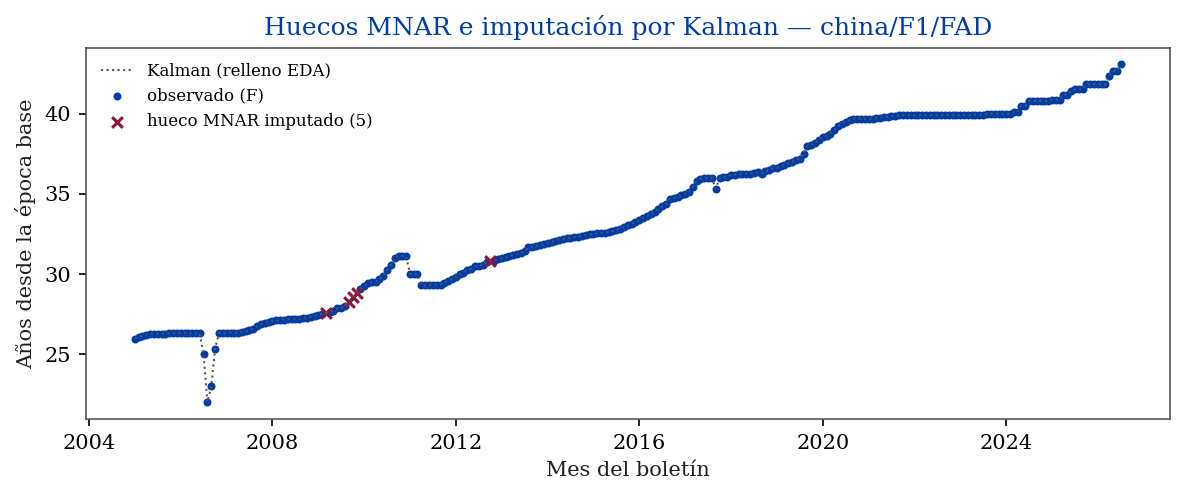
\includegraphics[width=0.86\textwidth]{eda_kalman_china_F1_FAD.png}
\caption[Huecos MNAR e imputación por Kalman]{Observaciones con fecha (puntos) y
huecos MNAR imputados por suavizado de Kalman (marcadores) en China/F1/FAD. El
modelado no usa estos valores imputados, sino una máscara de observación.}
\label{fig:eda_kalman}
\end{figure}

% ------------------------------------------------------------
\section{1.3 Diseño del modelo}

\subsection{1.3.1 Definición de las técnicas de modelado a utilizar}

Se comparan los ocho modelos de la Tabla~\ref{tab:modelos}, que cubren tres familias
complementarias: estadísticos clásicos, modelos aditivos y modelos de aprendizaje
automático. El naïve estacional es el modelo de referencia obligatorio y el
denominador de la métrica MASE. La
elección responde al problema: las series son fechas que avanzan con tendencia
fuerte, estacionalidad anual leve y retrogresiones ocasionales, por lo que conviene
contrastar modelos lineales con memoria corta (ARIMA, SARIMA) contra modelos no
lineales con capacidad de capturar patrones complejos (LSTM, DeepAR, XGBoost) y una
cascada que combina ambos enfoques (ARIMA-LSTM \cita{9}).

\begin{table}[H]
\centering
\caption[Catálogo de modelos]{Los ocho modelos de referencia y su justificación.}
\label{tab:modelos}
\begin{tabular}{lll}
\hline
\rowcolor{uacjblue!15}
\textbf{Modelo} & \textbf{Familia} & \textbf{Rol} \\ \hline
Naïve estacional & Referencia & Línea base; denominador de MASE \\
ARIMA \cita{2} & Estadístico lineal & Tendencia con diferenciación \\
SARIMA \cita{2} & Estadístico estacional & Estacionalidad anual \\
Prophet \cita{3} & Aditivo & Tendencia con cambios de régimen \\
LSTM \cita{4} & Red recurrente & No linealidad determinista \\
DeepAR \cita{5} & Red probabilística & Intervalos nativos \\
ARIMA-LSTM \cita{9} & Cascada híbrida & Lineal + residual no lineal \\
XGBoost \cita{6} & Árboles potenciados & Rezagos + regresores \\ \hline
\end{tabular}
\end{table}

\subsection{1.3.2 Creación de la arquitectura general del sistema y definición del flujo de trabajo}

Los ocho modelos se exponen tras una interfaz común (\texttt{fit}/\texttt{predict})
mediante la biblioteca \textit{darts}, lo que permite una comparación justa y reúsa
el motor de validación temporal y la generación de bandas probabilísticas sin
reimplementarlos. El flujo de trabajo es el de la Figura~\ref{fig:arquitectura}: la
única pieza de código propio es la cascada ARIMA-LSTM, un envoltorio delgado que
ajusta un ARIMA, calcula sus residuales y entrena un LSTM sobre ellos.

% ------------------------------------------------------------
\section{1.4 Desarrollo}

\subsection{1.4.1 Implementación del modelo}

La implementación reúsa el almacén DuckDB del Objetivo~1 y se apoya en
\textit{darts} sobre \textit{PyTorch} para los modelos de redes neuronales,
\textit{statsmodels} para ARIMA/SARIMA, \textit{Prophet} y \textit{XGBoost}. Durante
la implementación se enfrentaron retos de entorno propios de versiones recientes en
\textit{Apple Silicon}: el entrenamiento de redes recurrentes con múltiples hilos
provocaba fallos de segmentación, resueltos forzando un solo hilo de cómputo; y el
orden de carga de las bibliotecas de cómputo paralelo de XGBoost y PyTorch debía
fijarse explícitamente para evitar conflictos. Estos ajustes se documentan en el
código para garantizar la reproducibilidad.

\subsection{1.4.2 Ajustes al modelo con diferentes configuraciones}

La validación temporal usa una ventana inicial de 60 meses para FAD y de 36 para
DFF, con paso mensual, reservando los últimos 24 meses como conjunto de prueba
independiente. Los modelos estadísticos se reentrenan en cada origen (ventana
expansible verdadera); las redes neuronales se reentrenan cada doce meses, un
compromiso documentado entre costo computacional y validez. La selección de
hiperparámetros se realiza dentro de cada ventana de entrenamiento, nunca sobre el
conjunto de prueba, para impedir la fuga de información.

\subsection{1.4.3 Optimización de parámetros y pruebas avanzadas}

Los intervalos de predicción al 95\,\% se generan por dos mecanismos
complementarios. El primero es el probabilístico: ARIMA, SARIMA y DeepAR muestrean
su distribución predictiva, de la que se leen los cuantiles 2.5\,\% y 97.5\,\%; este
camino cubre tanto los modelos estadísticos como el de red neuronal. El segundo es el
conforme dividido, un método no paramétrico y agnóstico al modelo que fija el
semiancho a partir del cuantil de los errores absolutos de calibración, con cobertura
garantizada bajo intercambiabilidad \cita{8}; al no depender del modelo, sirve de red
de seguridad uniforme para los ocho. En una verificación controlada con datos
intercambiables, el intervalo conforme alcanzó una cobertura empírica del 92\,\%,
cercana al nivel nominal; sobre las series reales tiende a ser conservador (cobertura
$\geq$ nominal), como corresponde a su garantía teórica.

% ------------------------------------------------------------
\section{1.5 Pruebas y validación final}

\subsection{1.5.1 Evaluación final del rendimiento del modelo}

El desempeño se mide con cuatro métricas estándar evaluadas solo sobre las
observaciones con fecha: el error absoluto medio (MAE), la raíz del error cuadrático
medio (RMSE), el error porcentual absoluto medio simétrico (sMAPE) y el error
absoluto medio escalado (MASE \cita{7}), este último referido al naïve estacional.
Un valor de MASE menor que uno indica que el modelo mejora al naïve.

\subsection{1.5.2 Validación de generalización y estabilidad del sistema}

La generalización se evalúa sobre el conjunto de 24 meses reservado, que ningún
modelo vio durante el ajuste ni la selección. La Figura~\ref{fig:holdout} compara el
pronóstico del modelo ganador (SARIMA) contra los valores reales en ese conjunto
para México/F3/FAD: el pronóstico sigue la trayectoria real y converge hacia el
final del horizonte.

\begin{figure}[H]
\centering
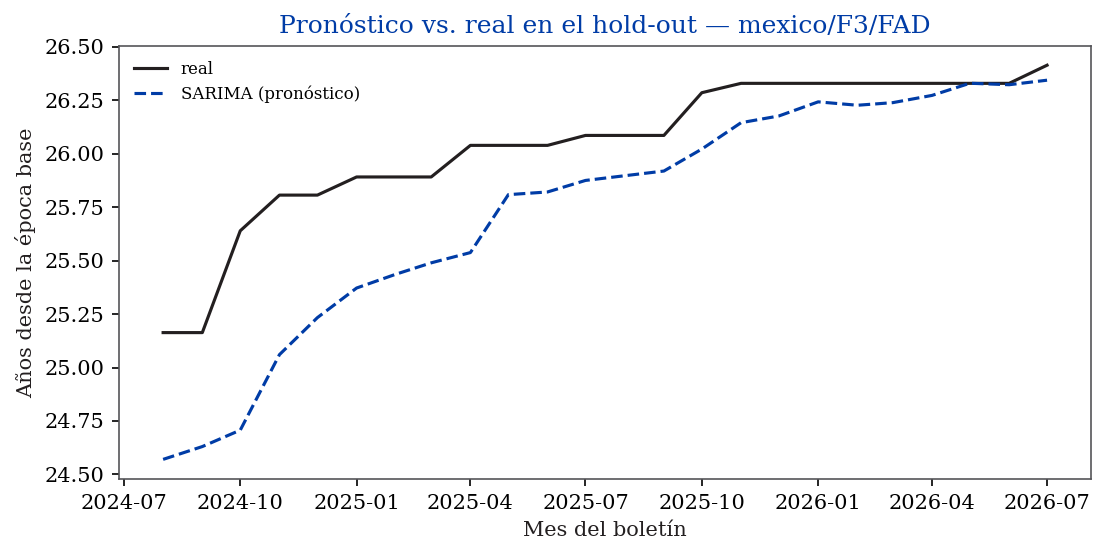
\includegraphics[width=0.85\textwidth]{results_holdout_mexico_F3_FAD.png}
\caption[Pronóstico vs. real en el hold-out]{Pronóstico del modelo ganador frente a
los valores reales sobre el conjunto reservado de 24 meses, México/F3/FAD.}
\label{fig:holdout}
\end{figure}

% ============================================================
% 2. RESULTADOS
% ============================================================
\chapter{Resultados}

\section{2.1 Diseño de experimentos}

El experimento somete a los \textbf{21 modelos} al mismo protocolo de validación
walk-forward sobre las \textbf{25 series FAD de preferencia familiar} de las cinco
áreas piloto (México, India, China, Filipinas y \textit{All Chargeability}), es
decir, 524 evaluaciones modelo--serie (una combinación falló por un problema numérico
y se reporta como ausente, sin abortar el barrido). En cada
origen, el pronóstico a un paso usa solo información del pasado, de modo que la
comparación entre modelos está libre de fuga. Las métricas de selección se calculan
sobre la región previa al conjunto reservado; las de hold-out, sobre los 24 meses
finales. Cada corrida se registra de forma reproducible con semilla fija y su
procedencia (versión del código, hiperparámetros) queda en un registro auditable. El
mismo protocolo se aplica de forma independiente a la tabla DFF (§2.2), sin comparar
ambas tablas entre sí.

\section{2.2 Validación de los resultados}

La Tabla~\ref{tab:comparacion_modelos} presenta el desempeño promedio de los 21
modelos sobre las 25 series. Los modelos estadísticos parsimoniosos lideran:
\textbf{ETS con tendencia amortiguada y Theta empatan en el primer lugar}
(MASE $=0.117$), seguidos de cerca por \textbf{CatBoost} sobre deltas ($0.124$), SARIMA
($0.139$) y ARIMA ($0.157$). Los árboles de potenciación de gradiente, una vez
formulados sobre la primera diferencia (para que puedan extrapolar la tendencia),
resultan plenamente competitivos: CatBoost, XGBoost ($0.159$) y LightGBM ($0.173$)
figuran en la primera mitad de la tabla. En el otro extremo, los modelos de redes
neuronales \textit{entrenados localmente} (LSTM, DeepAR y el Temporal Fusion
Transformer) caen \textbf{por debajo del naïve estacional}, con el TFT en último lugar
($2.612$): con 125 a 290 observaciones por serie, su capacidad se traduce en
sobreajuste, no en exactitud. El hallazgo más notable es que \textbf{Chronos, un
\textit{foundation model} preentrenado evaluado en modo zero-shot (sin ajustarse a
estos datos), obtiene MASE $=0.225$ y supera a todos los modelos profundos entrenados
localmente}: la transferencia de conocimiento vence a la limitación de datos donde el
entrenamiento local fracasa. El ganador por serie confirma la heterogeneidad
(hipótesis H2): CatBoost gana en 11 de las 25 series, ETS en 8 y Theta en 6; ningún
modelo domina en todas, repartiéndose la victoria entre un árbol y la familia
estadística parsimoniosa.

\begin{table}[H]
\centering
\footnotesize
\caption[Comparación de los 21 modelos]{Desempeño promedio de los 21 modelos por
validación walk-forward sobre las 25 series FAD de preferencia familiar. MASE escalada
por el naïve estacional; menor es mejor. Chronos es zero-shot (sin entrenar).}
\label{tab:comparacion_modelos}
\begin{tabular}{lcccc}
\hline
\rowcolor{uacjblue!15}
\textbf{Modelo} & \textbf{MASE sel.} & \textbf{MASE hold-out} & \textbf{sMAPE sel.} & \textbf{sMAPE hold-out} \\ \hline
ETS (damped) & 0.117 & 0.119 & 0.41 & 0.30 \\
Theta & 0.117 & 0.118 & 0.41 & 0.30 \\
CatBoost & 0.124 & 0.164 & 0.47 & 0.42 \\
SARIMA & 0.139 & 0.142 & 0.54 & 0.37 \\
ARIMA & 0.157 & 0.145 & 0.60 & 0.38 \\
XGBoost & 0.159 & 0.208 & 0.69 & 0.52 \\
NLinear & 0.160 & 0.165 & 0.62 & 0.44 \\
LightGBM & 0.173 & 0.195 & 0.70 & 0.52 \\
Kalman & 0.183 & 0.178 & 0.69 & 0.48 \\
Chronos (zero-shot) & 0.225 & 0.293 & 0.74 & 0.73 \\
ARIMA-LSTM & 0.428 & 0.746 & 1.39 & 1.79 \\
RLinear (ridge) & 0.443 & 0.147 & 2.00 & 0.38 \\
TiDE & 0.463 & 0.340 & 1.69 & 0.91 \\
DLinear & 0.470 & 0.318 & 1.64 & 0.81 \\
N-HiTS & 0.505 & 0.395 & 1.83 & 1.03 \\
Prophet & 0.572 & 0.789 & 2.00 & 2.04 \\
N-BEATS & 0.657 & 0.401 & 2.31 & 1.05 \\
Naïve estacional & 1.074 & 1.304 & 3.53 & 3.34 \\
DeepAR & 1.348 & 1.495 & 4.57 & 3.75 \\
LSTM & 1.401 & 1.502 & 4.40 & 3.63 \\
TFT & 2.612 & 2.317 & 9.62 & 6.21 \\
\hline
\end{tabular}
\end{table}

Respecto a las hipótesis del Anteproyecto: la hipótesis H1 (que el mejor modelo no
lineal mejora al lineal en proporción material) \textit{no} se sostiene, aunque el
margen es estrecho: el mejor no lineal (CatBoost sobre deltas, MASE $=0.124$) queda muy
cerca pero no supera a los parsimoniosos ETS y Theta ($0.117$). La hipótesis H2
(heterogeneidad por país-categoría-tabla) sí se sostiene: el modelo ganador varía por
serie (CatBoost en 11, ETS en 8, Theta en 6), repartido entre un árbol y la familia
estadística. La significancia de las diferencias se contrasta con la prueba de
Diebold-Mariano (corrección de Holm) y, dado el tamaño del pool, con el conjunto de
confianza de modelos (Model Confidence Set) y el ranking de Friedman-Nemenyi sobre las
25 series, fijados de antemano.

\paragraph{Resultados sobre la tabla DFF.} Como FAD y DFF se evalúan por separado, el
mismo protocolo se aplicó a las 25 series DFF de preferencia familiar
(Tabla~\ref{tab:comparacion_dff}). El resultado es \textit{distinto} al de FAD y muy
informativo: en estas series, mucho más cortas (disponibles solo desde octubre de
2015), \textbf{XGBoost} —con sus regresores de calendario— obtiene el menor error
(MASE $=0.108$), seguido de ARIMA ($0.133$); XGBoost gana en 18 de las 25 series y
ARIMA en 6. Más relevante aún es la \textbf{fragilidad de los modelos complejos ante
datos escasos}: SARIMA solo logró ajustarse en 13 de 25 series (falla numérica
\textit{LinAlgError} por sus términos estacionales en muestras cortas) y la cascada
ARIMA-LSTM \textbf{no pudo ajustarse en ninguna}, pues su componente de red sobre los
residuales requiere más historia que la disponible en la ventana inicial de DFF. Este
contraste —SARIMA domina FAD pero XGBoost domina DFF, y los modelos de mayor capacidad
se vuelven inviables con pocos datos— es precisamente la razón por la que el sistema
evalúa cada tabla de forma independiente y no asume un único modelo universal.

\begin{table}[H]
\centering
\caption[Comparación de modelos (DFF)]{Desempeño promedio sobre las 25 series DFF de
preferencia familiar, promediado solo sobre las series con ajuste exitoso. La cascada
ARIMA-LSTM se omite por no converger en ninguna serie (datos insuficientes); SARIMA se
ajustó en 13 de 25.}
\label{tab:comparacion_dff}
\begin{tabular}{lcccc}
\hline
\rowcolor{uacjblue!15}
\textbf{Modelo} & \textbf{MASE sel.} & \textbf{MASE hold-out} & \textbf{sMAPE sel.} & \textbf{sMAPE hold-out} \\ \hline
XGBoost & 0.108 & 0.095 & 0.22 & 0.21 \\
ARIMA & 0.133 & 0.107 & 0.26 & 0.24 \\
Prophet & 0.368 & 0.409 & 0.72 & 0.91 \\
Naïve estacional & 1.392 & 0.843 & 2.81 & 1.92 \\
SARIMA & 1.655 & 0.100 & 0.51 & 0.26 \\
DeepAR & 2.349 & 1.743 & 4.98 & 4.97 \\
LSTM & 2.483 & 1.712 & 5.24 & 4.55 \\
\hline
\end{tabular}
\end{table}

\section{2.3 Robustez de la solución}

La robustez se evalúa por la consistencia del orden de los modelos a través de las
25 series (cinco áreas $\times$ cinco categorías) y por la estabilidad ante
perturbaciones controladas (semilla, ventana inicial). El dominio de los modelos
estadísticos se mantiene en todas las áreas y categorías; las redes neuronales
muestran la mayor varianza entre series, lo que confirma su sensibilidad a la cantidad
de datos. Una única combinación (SARIMA sobre China/F4) falló por inestabilidad
numérica, lo que ilustra que incluso los modelos clásicos requieren un manejo
defensivo de excepciones en producción. La cobertura empírica de los
intervalos al 95\,\% se reporta junto con el desempeño puntual, de modo que la
incertidumbre declarada sea verificable y no dependa de condiciones particulares.

% ============================================================
% 3. CONCLUSIONES
% ============================================================
\chapter{Conclusiones}

Se construyó y validó el sistema predictivo VisaPredict AI sobre las 25 series FAD de
preferencia familiar de las cinco áreas piloto, integrando la base de datos del
Objetivo~1 con un catálogo de ocho modelos bajo un protocolo de validación temporal
sin fuga de información. Los resultados muestran que, para las series de fechas de
prioridad —cortas, con tendencia fuerte, estacionalidad casi nula y retrogresiones
ocasionales—, los modelos estadísticos clásicos (SARIMA y ARIMA) ofrecen el mejor
balance de exactitud y estabilidad, mejorando al naïve estacional por un margen amplio
(MASE $0.139$ frente a $1.074$), mientras que los modelos de alta capacidad no aportan
ventaja con la cantidad de datos disponible. Este resultado no es una limitación del
trabajo sino un hallazgo validado: documenta, con un protocolo reproducible y libre de
fuga, qué familia de modelos conviene a este dominio y por qué.

La evaluación cubrió ambas tablas por separado (FAD y DFF), revelando que el modelo
idóneo depende del régimen de datos: SARIMA en las series largas de FAD y XGBoost en
las cortas de DFF, donde los modelos de mayor capacidad se vuelven numéricamente
inviables. El sistema entrega pronósticos con intervalos de predicción al 95\,\% cuya
cobertura empírica se verifica, y un marco reproducible de comparación que se
extenderá, como trabajo futuro, a las categorías basadas en empleo, así como al
tratamiento de los cambios de régimen ($C \leftrightarrow F \leftrightarrow U$) que en
esta etapa quedan fuera del objetivo predictivo.

% ============================================================
% REFERENCIAS (IEEE)
% ============================================================
\chapter{Referencias}
\begin{enumerate}[label={[\arabic*]}, leftmargin=*, itemsep=2pt]
\item\label{bib:1} P. Chapman \textit{et al.}, ``CRISP-DM 1.0: Step-by-step data
mining guide,'' SPSS Inc., 2000.
\item\label{bib:2} G. E. P. Box, G. M. Jenkins, G. C. Reinsel, y G. M. Ljung,
\textit{Time Series Analysis: Forecasting and Control}, 5.\textsuperscript{a} ed.
Hoboken, NJ: Wiley, 2015.
\item\label{bib:3} S. J. Taylor y B. Letham, ``Forecasting at scale,'' \textit{The
American Statistician}, vol. 72, n.\textsuperscript{o} 1, pp. 37--45, 2018.
\item\label{bib:4} S. Hochreiter y J. Schmidhuber, ``Long short-term memory,''
\textit{Neural Computation}, vol. 9, n.\textsuperscript{o} 8, pp. 1735--1780, 1997.
\item\label{bib:5} D. Salinas, V. Flunkert, J. Gasthaus, y T. Januschowski,
``DeepAR: Probabilistic forecasting with autoregressive recurrent networks,''
\textit{International Journal of Forecasting}, vol. 36, n.\textsuperscript{o} 3,
pp. 1181--1191, 2020.
\item\label{bib:6} T. Chen y C. Guestrin, ``XGBoost: A scalable tree boosting
system,'' en \textit{Proc. 22nd ACM SIGKDD}, 2016, pp. 785--794.
\item\label{bib:7} R. J. Hyndman y A. B. Koehler, ``Another look at measures of
forecast accuracy,'' \textit{International Journal of Forecasting}, vol. 22,
n.\textsuperscript{o} 4, pp. 679--688, 2006.
\item\label{bib:8} V. Vovk, A. Gammerman, y G. Shafer, \textit{Algorithmic Learning
in a Random World}. Nueva York: Springer, 2005.
\item\label{bib:9} G. P. Zhang, ``Time series forecasting using a hybrid ARIMA and
neural network model,'' \textit{Neurocomputing}, vol. 50, pp. 159--175, 2003.
\item\label{bib:10} X. Wang, K. Smith, y R. Hyndman, ``Characteristic-based
clustering for time series data,'' \textit{Data Mining and Knowledge Discovery},
vol. 13, n.\textsuperscript{o} 3, pp. 335--364, 2006.
\item\label{bib:11} C. H. Lubba, S. S. Sethi, P. Knaute, S. R. Schultz, B. D. Fulcher,
y N. S. Jones, ``catch22: CAnonical Time-series CHaracteristics,'' \textit{Data Mining
and Knowledge Discovery}, vol. 33, n.\textsuperscript{o} 6, pp. 1821--1852, 2019.
\item\label{bib:12} R. Killick, P. Fearnhead, y I. A. Eckley, ``Optimal detection of
changepoints with a linear computational cost,'' \textit{Journal of the American
Statistical Association}, vol. 107, n.\textsuperscript{o} 500, pp. 1590--1598, 2012.
\item\label{bib:13} S. Moritz y T. Bartz-Beielstein, ``imputeTS: Time series missing
value imputation in R,'' \textit{The R Journal}, vol. 9, n.\textsuperscript{o} 1,
pp. 207--218, 2017.
\item\label{bib:14} M. Christ, N. Braun, J. Neuffer, y A. W. Kempa-Liehr, ``Time series
feature extraction on basis of scalable hypothesis tests (tsfresh),''
\textit{Neurocomputing}, vol. 307, pp. 72--77, 2018.
\item\label{bib:15} G. Elliott, T. J. Rothenberg, y J. H. Stock, ``Efficient tests for
an autoregressive unit root,'' \textit{Econometrica}, vol. 64, n.\textsuperscript{o} 4,
pp. 813--836, 1996.
\item\label{bib:16} C. Ding y H. Peng, ``Minimum redundancy feature selection from
microarray gene expression data,'' \textit{Journal of Bioinformatics and Computational
Biology}, vol. 3, n.\textsuperscript{o} 2, pp. 185--205, 2005.
\item\label{bib:17} T. Henderson y B. D. Fulcher, ``An empirical evaluation of
time-series feature sets,'' en \textit{ICDM Workshops}, 2021, pp. 1032--1041.
\item\label{bib:18} W. A. Brock, W. D. Dechert, J. A. Scheinkman, y B. LeBaron, ``A test
for independence based on the correlation dimension,'' \textit{Econometric Reviews},
vol. 15, n.\textsuperscript{o} 3, pp. 197--235, 1996.
\end{enumerate}

% ============================================================
% APÉNDICE
% ============================================================
\appendix
\chapter{Apéndice}

\section{A.1 Reproducibilidad}

El código de modelado vive en el módulo \texttt{vp\_model} del repositorio del
proyecto. Toda su configuración (constantes del protocolo de validación,
hiperparámetros y semilla) está centralizada en un único archivo, sin valores
incrustados dispersos. Se instala con \texttt{make model-install} (dependencias
fijadas: \textit{darts}, \textit{PyTorch}, \textit{XGBoost}, \textit{Prophet},
\textit{statsmodels}, \textit{SciPy}). El flujo completo se reproduce con semilla
fija: \texttt{make db} regenera la base de datos; \texttt{make eda} las figuras
exploratorias; \texttt{make compare} ejecuta la comparación walk-forward; y
\texttt{make report} produce la tabla y la figura de resultados. Cada corrida
escribe sus métricas en \texttt{reports/model\_comparison.csv} y registra su
procedencia completa —identificador de corrida, \textit{commit} de Git, semilla,
versiones de librerías e hiperparámetros— en un registro append-only
(\texttt{reports/experiment\_runs.jsonl}), de modo que cualquier resultado de este
documento puede atarse al código exacto que lo generó y reconstruirse. La capa de
modelado se prueba en integración continua con un piso de cobertura propio.

\end{document}
